\documentclass[border=3mm]{standalone}
\usepackage{tikz}
\usetikzlibrary{circuits.logic.US}

\begin{document}
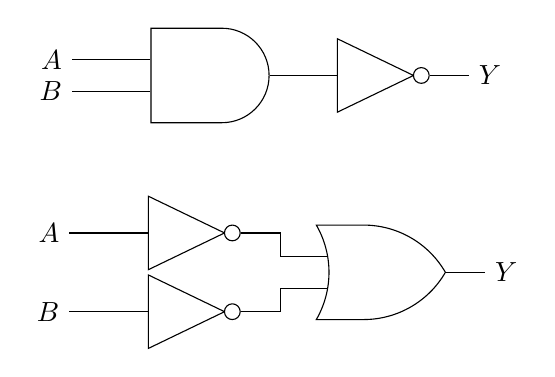
\begin{tikzpicture}[circuit logic US,
                    tiny circuit symbols,
                    every circuit symbol/.style={fill=white,draw,logic gate input sep=4mm, logic gate inverted radius=1mm}
]

\node [and gate, inputs = nn] at (0,0) (and1) {};
\node [not gate, inputs = n] at ($(and1) + (2.0cm,0)$) (not1) {};
\draw (and1.input 1) -- ++(left:10mm) node[left] (A) {$A$};
\draw (and1.input 2) -- ++(left:10mm) node[left] (B) {$B$};
\draw (and1.output) -- ++(right:5mm) |- (not1.input);
\draw (not1.output) -- ++(right:5mm) node[right] (Y) {$Y$};
%
\node [not gate, inputs = n] at (-0.4,-2) (not2) {};
\node [not gate, inputs = n] at (-0.4,-3) (not3) {};
\node [or gate, inputs = nn] at ($(not2) + (2.5cm,-0.5cm)$) (or1) {};
\draw (not2.input) -- ++(left:10mm) node[left] (C) {$A$};
\draw (not3.input) -- ++(left:10mm) node[left] (D) {$B$};
\draw (not2.output) -- ++(right:5mm) |- (or1.input 1);
\draw (not3.output) -- ++(right:5mm) |- (or1.input 2);
\draw (or1.output) -- ++(right:5mm) node[right] (Q) {$Y$};

\end{tikzpicture}
\end{document}
